\documentclass[a4paper, 12pt]{article}

\usepackage{xeCJK}
\setCJKmainfont{Songti SC}
\usepackage{fontspec}
\setmainfont{Times New Roman}
\usepackage{fullpage}
\usepackage{setspace}
\onehalfspacing
\usepackage{indentfirst}
\setlength{\parindent}{2em}
\usepackage{graphicx}

\begin{document}
\title{{\Large SoCaffe: 基于Zynq SoC平台的高性能深度学习框架}}
\author{{\large 信息科学技术学院}\\{\large 赵睿哲}\\{\large 1200012778}}
\date{}
\maketitle

\section{摘要}
近年来,深度学习与神经网络领域飞速发展,并逐渐应用于无人机、自动驾驶汽车等平台。这类平台使用嵌入式设备进行计算,对功耗、算法的实时性、计算资源都有一定的限制,与传统的深度学习应用所依赖的GPU或者集群在性能上相差甚远。因此直接移植深度学习应用到嵌入式设备有很大的难度。

本研究实现了SoCaffe—一个基于Caffe与和Zynq SoC的深度学习框架。
Caffe作为最流行的CPU/GPU深度学习框架之一,效率高、配置简单,并为大部分研究人员所熟悉。Zynq SoC是Xilinx公司推出的“全可编程”嵌入式开发平台,搭载高效的ARM Cortex-A9双核CPU与Xilinx FPGA,能同时满足计算性能与功耗比的要求。

本研究综合考虑了Zynq SoC平台的特点与Caffe的计算特性,
对Caffe的功能进行软硬件逻辑划分,挑选Caffe中密集使用的GEMM计算作为FPGA加速的目标。针对GEMM的硬件逻辑设计,本研究对其性能进行了细致的分析和数学建模,从硬件资源占用与延迟两个角度进行了充分的优化,达到了相对于软件版本5.4x加速比和最高12.31GFLOPS的性能。同时,本研究生成的SoCaffe框架的功能基本与Caffe完全一致,基于其他硬件平台的Caffe应用可以直接移植到Zynq SoC上实现。最后,SoCaffe的整体计算性能也有最高2.34x的加速比。此外,本研究完全基于Xilinx新推出的SDSoC开发平台进行软硬件协同设计,大大提升了开发效率。

综上,SoCaffe同时拥有Zynq SoC平台的高性能与Caffe框架的通用性和易用性,是针对嵌入式平台深度学习应用开发的实际解决方案,具有一定的实用价值。

\section{主要工作}
本研究的主要工作如下:
\begin{enumerate}
	\item 使用Vivado HLS工具实现了GEMM计算在FPGA上的设计与实现,针对Zynq-7000的系统资源特点给出了相应的优化方案与数学分析模型,找到了能实现的矩阵块大小的上界;同时使用了半精度浮点数优化了对计算资源的使用。最终获得最高12.31GFLOPS和5.42倍加速比。
	\item 系统地学习和掌握了Xilinx SDSoC开发环境的使用方式,通过文档与探索自主掌握了该工具的高级使用方法,并针对SoCaffe的特点定制了一套开发流程。
	\item 使用ARM GNU工具链使用交叉编译的方式编译了全部Caffe需要使用的第三方库,使用SDSoC构建了SoCaffe的系统镜像文件包和动态链接库。
	\item 测试了SoCaffe的计算性能,可用性,精度等等特性,找到了SoCaffe的最佳使用条件:即针对大量使用卷积神经网络,网络规模较大的时候,SoCaffe可以取得不错的加速比。
\end{enumerate}

\section{未来工作}
SoCaffe存在一些缺点和亟待提高的地方:
1) 首先,因为Zynq SoC平台的内存有限,SoCaffe无法支持特别大的神经网络结构;
2) 其次,SoCaffe的GEMM固定块算法依然有一定的比重是冗余计算,如果输入矩阵形状比较小,则会造成较大比例的性能损失;
3) 最后,SoCaffe目前只支持GEMM的优化,其他不用到GEMM操作的网络层不能得到相应的性能提升。这些工作都是本研究下一步要进行优化的工作。

\section{测试数据}

\begin{figure}[!ht]
	\centering
	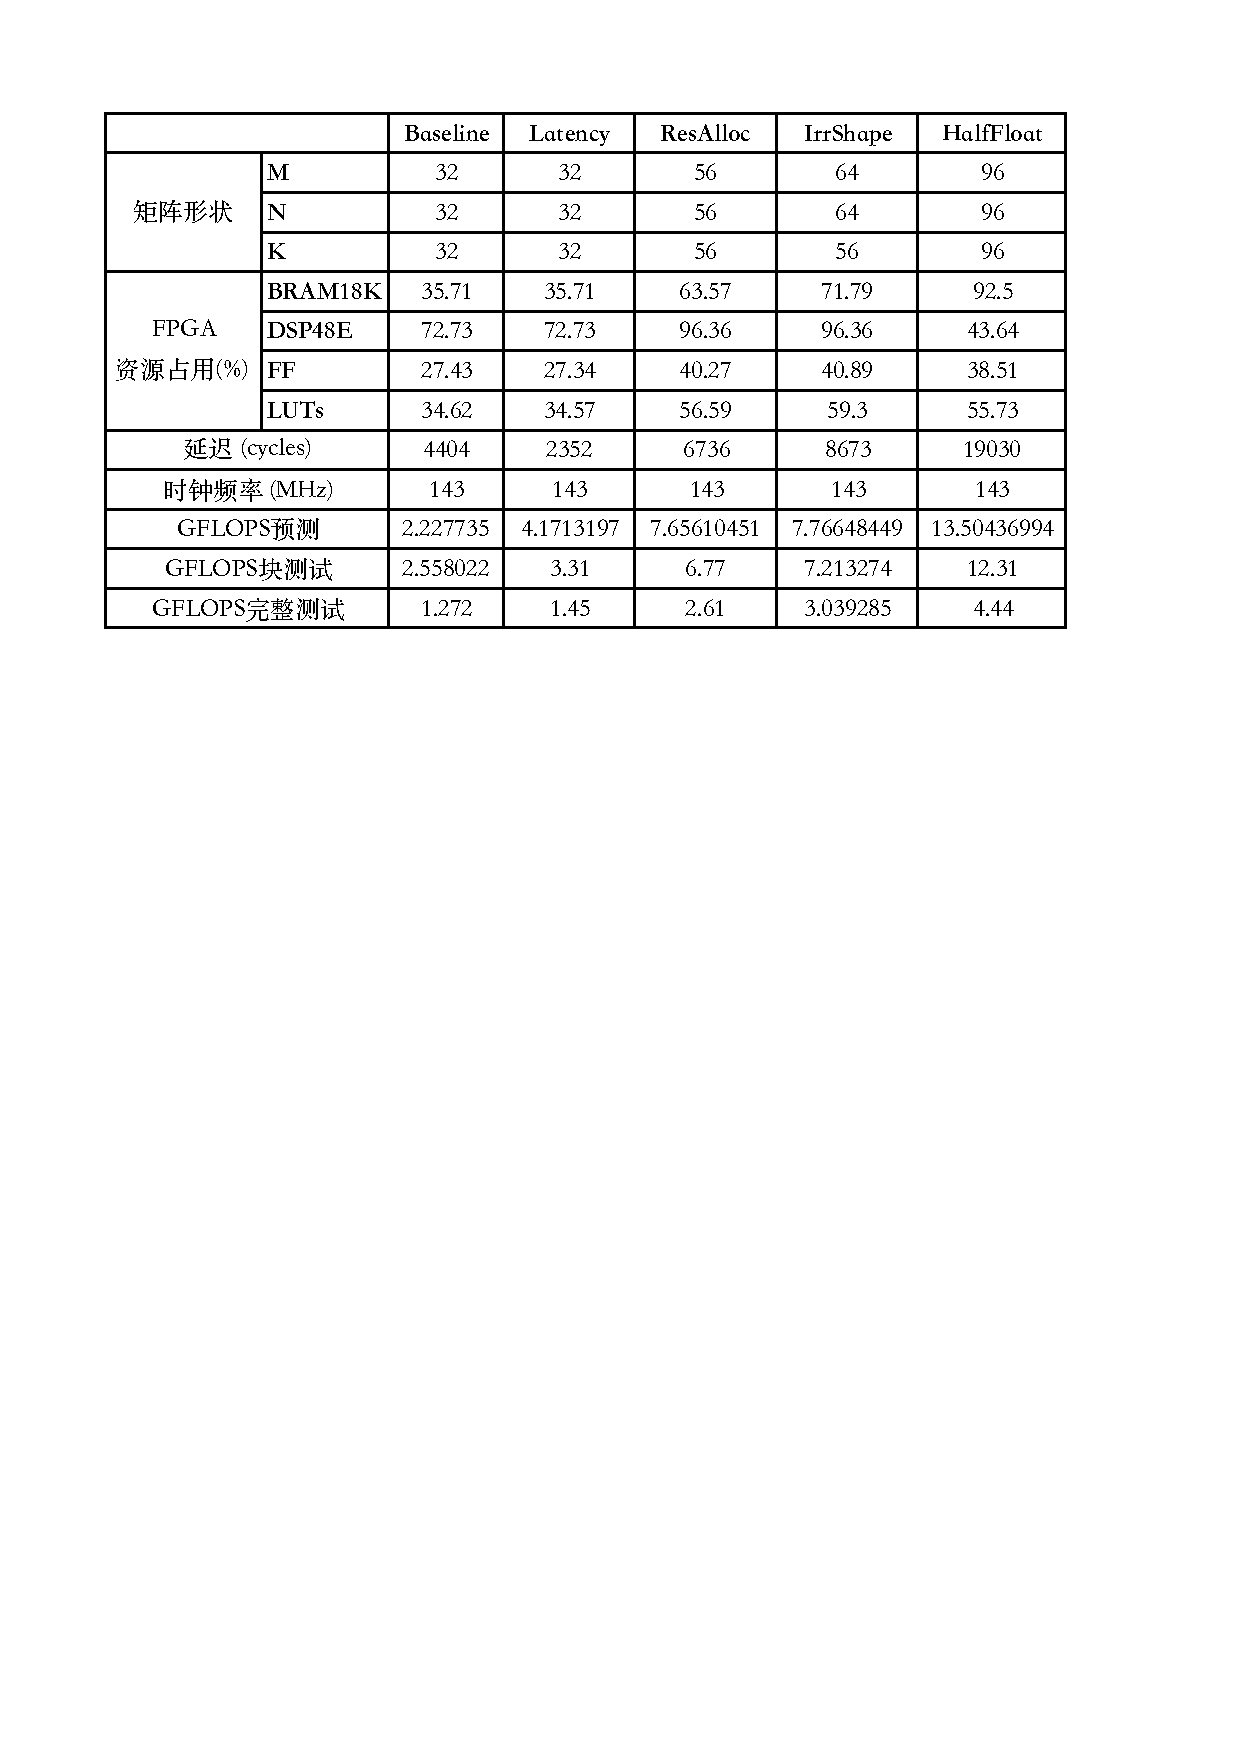
\includegraphics[width=0.8\textwidth]{assets/imgs/gemmcomp}
	\caption{GEMM的多种优化策略对比}
\end{figure}
\begin{figure}[!ht]
	\centering
	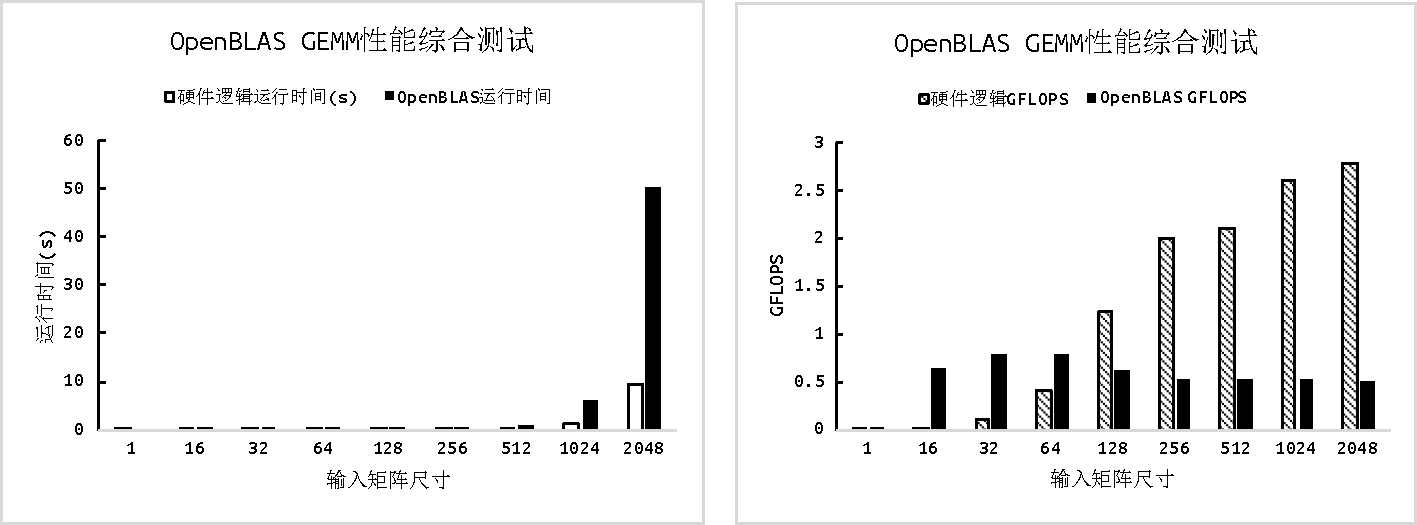
\includegraphics[width=0.8\textwidth]{assets/imgs/gemmblas}
	\caption{GEMM硬件加速与OpenBLAS版本的对比}
\end{figure}
\begin{figure}[!ht]
	\centering
	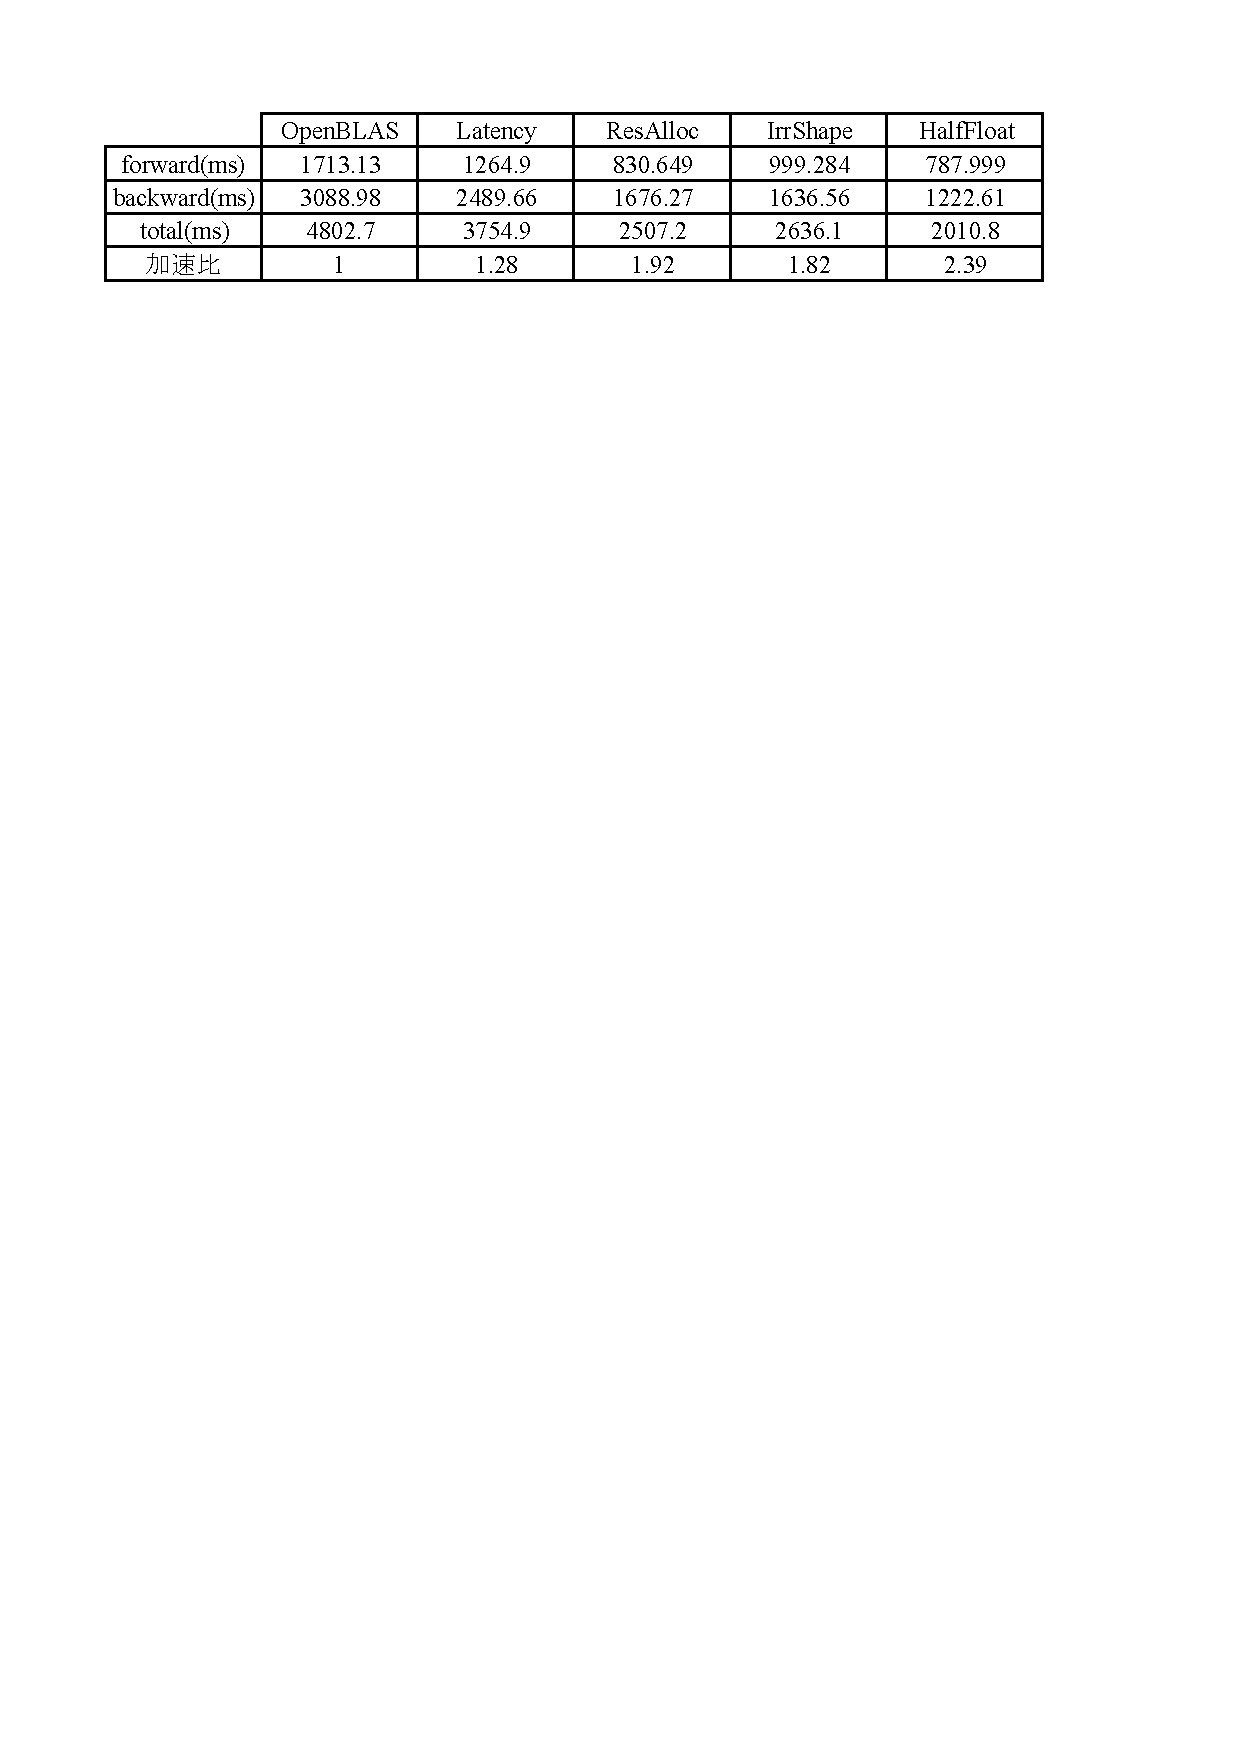
\includegraphics[width=0.8\textwidth]{assets/imgs/caffeconv}
	\caption{SoCaffe卷积层速度测试}
\end{figure}
\begin{figure}[!ht]
	\centering
	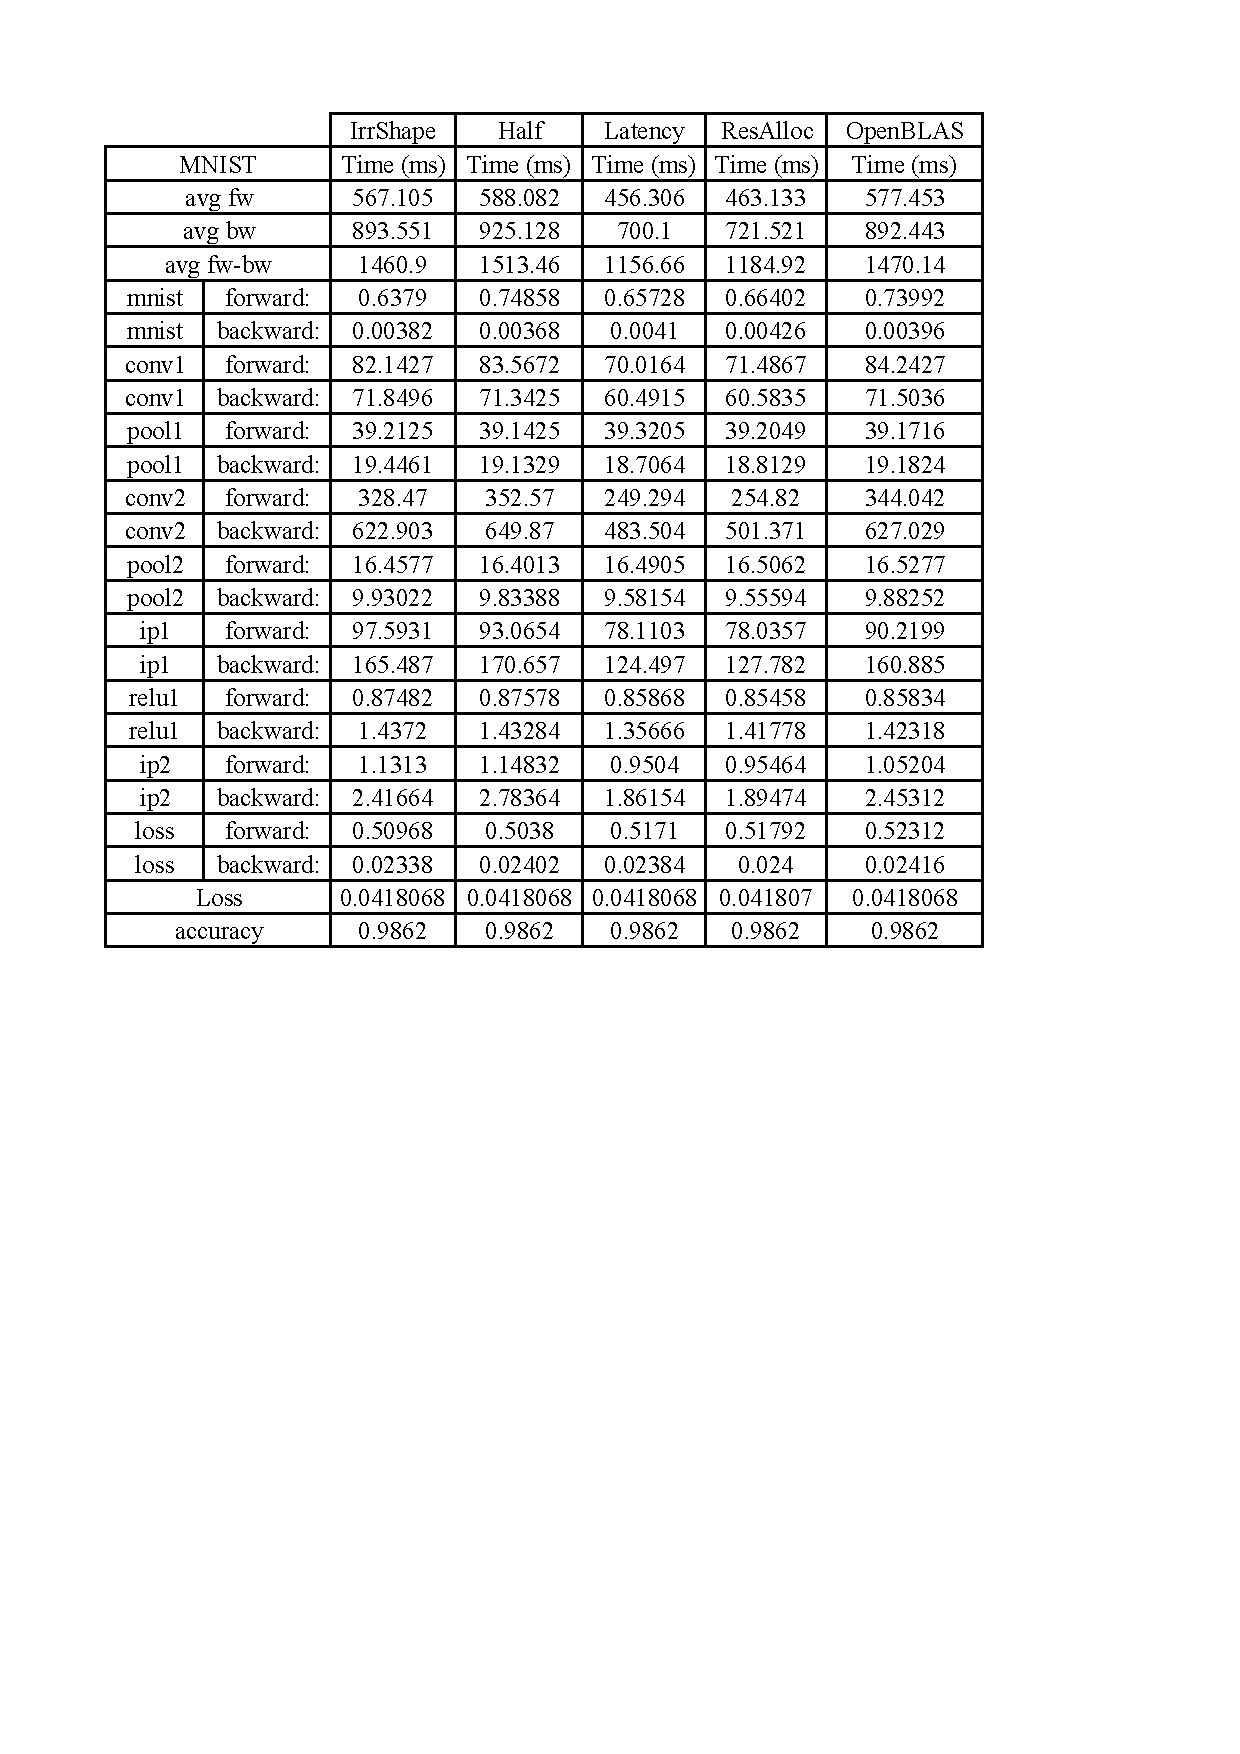
\includegraphics[width=0.8\textwidth]{assets/imgs/mnist}
	\caption{SoCaffe MNIST速度测试}
\end{figure}

\end{document}

